\chapter{Mengenal Python dan Anaconda}
Tujuan pembelajaran pada pertemuan pertama antara lain:
\begin{enumerate}
\item
Mengerti sejarah python, perkembangan dan penggunaan python di perusahaan
\item
Memahami tahapan instalasi python dan anaconda
\item
Memahami cara penggunaan spyder
\end{enumerate}
Tugas dengan cara dikumpulkan dengan pull request ke github dengan menggunakan format latex pada repo yang dibuat oleh asisten IRC.

\section{Teori}
Praktek teori penunjang yang dikerjakan :
\begin{enumerate}
\item
Buat Resume Sejarah Python, perbedaan python 2 dan 3, dengan bahasa yang mudah dipahami dan dimengerti. Buatan sendiri bebas plagiat(10)
\item
Buat Resume Implementasi dan penggunaan Python di perusahaan dunia, bahasa yang mudah dipahami(10)
\end{enumerate}

\section{Instalasi}
Melakukan instalasi python dan anaconda versi 3 serta uji coba spyder. Dengan menggunakan bahasa yang mudah dimengerti dan bebas plagiat. 
Dan wajib skrinsut dari komputer sendiri.
\begin{enumerate}
\item
Instalasi python 3 (5)
\item
instalasi pip(5)
\item
cara setting environment (5)
\item
mencoba entrepreter/cli melakui terminal atau cmd windows(5)
\item 
Menjalankan dan mengupdate anaconda dan spyder(5)
\item
Cara menjalankan Script hello word di spyder(5)
\item
Cara menjalankan Script otomatis login aplikasi akademik dengan library selenium dan inputan user(5)
\item
Cara pemakaian variable explorer di spyder(5)
\end{enumerate}


\section{Identasi}
Membuat file main.py dan mengisinya dengan script contoh python penggunaan selenium(minimal 20 baris) yang melibatkan inputan user, kemudian mencoba untuk mengatasi error identasi.
\begin{enumerate}
	\item
Penjelasan Identasi (10)
	\item
jenis jenis error identasi yang didapat(10)
\item
cara membaca error(10)
\item 
cara menangani errornya(10)
\end{enumerate}

\section{Presentasi Tugas}
Pada pertemuan ini, diadakan tiga penilaiain yaitu penilaian untuk tugas mingguan dengan nilai maksimal 100. Kemudian dalam satu minggu kedepan maksimal sebelum waktu mata kuliah. Ada presentasi kematerian dengan nilai presentasi yang terpisah masing-masing 100. Dan nilai terpisah untuk tutorial dari jawaban tugas di YouTube.Jadi ada tiga komponen penilaiain pada pertemuan ini yaitu :
\begin{enumerate}
	\item tugas minggu hari ini dan besok (maks 100). pada chapter ini
	\item presentasi csv (maks 100). Mempraktekkan kode python dan menjelaskan cara kerjanya.
	\item pembuatan video tutorial youtube tentang tutorial dari jawaban tugas.(nilai maks 100)
\end{enumerate}
Waktu presentasi pada jam kerja di IRC. Kriteria penilaian presentasi sangat sederhana, presenter akan ditanyai 20(10 pertanyaan program, 10 pertanyaan teori) pertanyaan tentang pemahamannya menggunakan python dan program agan dibuat error hingga presenter bisa menyelesaikan errornya. jika presenter tidak bisa menjawab satu pertanyaan asisten maka nilai nol. Jika semua pertanyaan bisa dijawab maka nilai 100. Presentasi bisa diulang apabila gagal, sampai bisa mendapatkan nilai 100 dalam waktu satu minggu kedepan.
\item \textbf{JAWABAN CHAPTER 1} 
\par
\textbf{Teori}
\begin{enumerate}
    \item Python diciptakan oleh Guido van Rossum pertama kali di  Centrum Wiskunde & Informatica (CWI) di Belanda pada awal tahun 1990-an. Bahasa python terinspirasi dari bahasa pemrograman ABC. 
\par
Pada tahun 1995, Guido melanjutkan pembuatan python di Corporation for National Research Initiative (CNRI) di Virginia Amerika, di mana dia merilis beberapa versi dari python.
\par
Pada Mei 2000, Guido dan tim Python pindah ke BeOpen.com dan membentuk tim BeOpen PythonLabs. Pada bulan Oktober pada tahun yang sama, tim python pindah ke Digital Creation (sekarang menjadi Perusahaan Zope). Di tahun 2001, dibentuklah Organisasi Python yaitu Python Software Foundation (PSF).
\par
Semua versi python yang dirilis bersifat open source. Dalam sejarahnya, hampir semua rilis python memakai lisensi GFL-compatible.
\par
perbedaan python 2 dan 3 yaitu Python 2 dinilai lebih transparan dan inklusif untuk pengembangan software ketimbang versi sebelumnya. Hal ini didukung dengan adanya PEP – Python Enhancement Proposal, sedangkan Python 3 itu sendiri berfokus untuk melakukan perapian pada codebase dan menghapuskan duplikasi (redundancy).

\item Beberapa platform populer seperti Spotify dan Netflix adalah contoh platform yang telah memanfaatkan Python dalam analisis data. Tim Spotify memanfaatkan analitis. Mereka memanfaatkan Luigi, modul dari Python, yang disinkronisasi dengan Hadoop, sebuah framework berbasis Java yang memungkinkan pemrosesan data dengan ukuran sangat besar.
\end{enumerate}
\textbf{Instalasi}
\begin{enumerate}
    \item Instalasi Python 3
    \begin{itemize}
        \item Jalankan instalasi terlebih dahulu, ceklis yang ada bacaan PATH, lalu klik install now \ref{proses1}
        \begin{figure} [h]
            \centering
            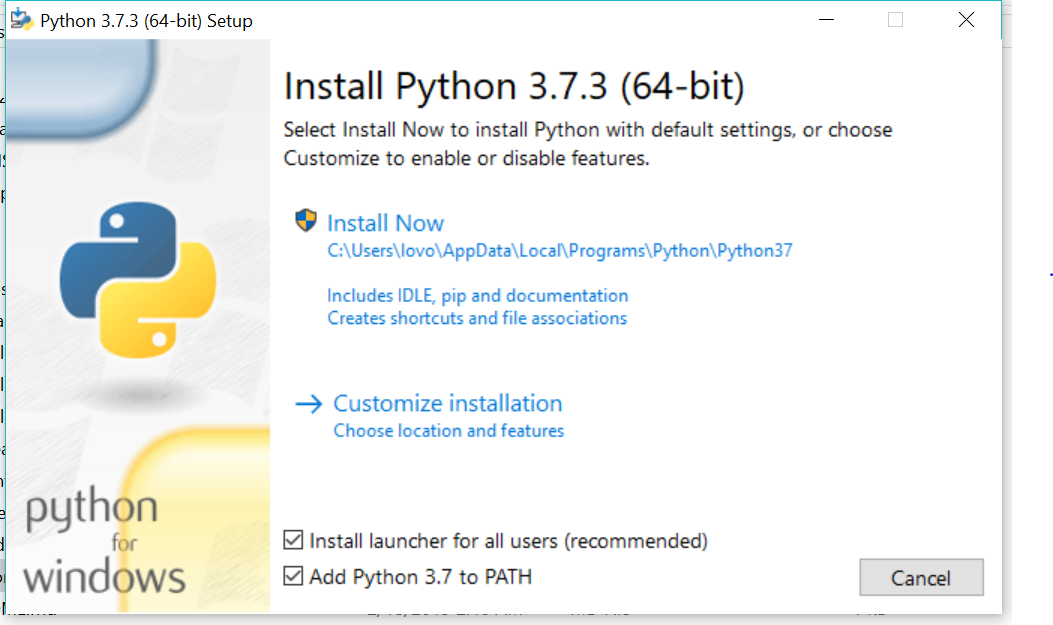
\includegraphics[scale=0.5]{figures/Capture1.PNG}
            \caption{Caption}
            \label{proses1}
        \end{figure}
        
        \item Tunggu progress hingga beres \ref{proses2}
        \begin{figure} [h]
            \centering
            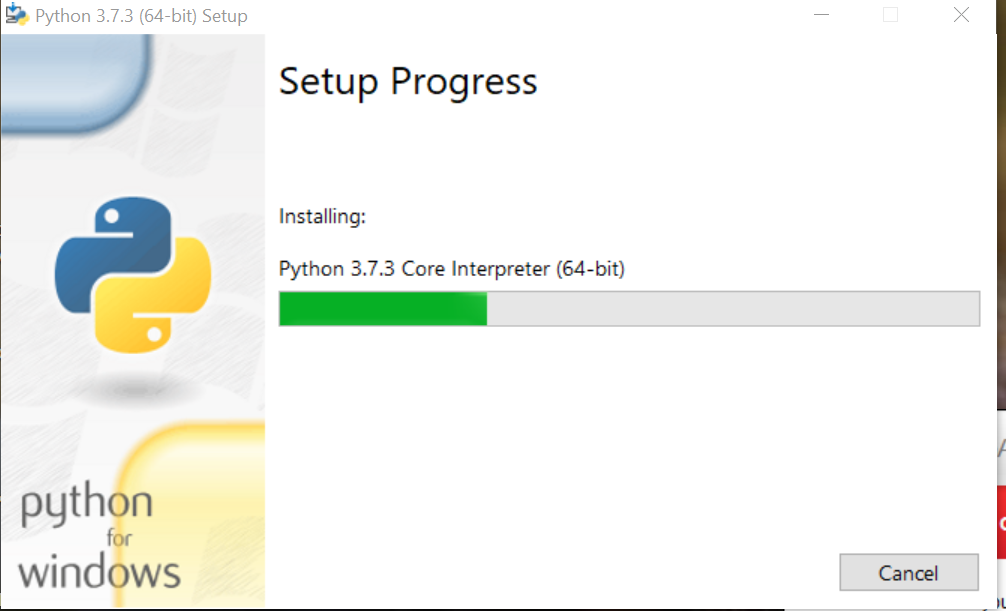
\includegraphics[scale=0.5]{figures/Capture2.PNG}
            \caption{Caption}
            \label{proses2}
        \end{figure}
        
        \item Instalasi selesai \ref{proses3}
        \begin{figure} [h]
            \centering
            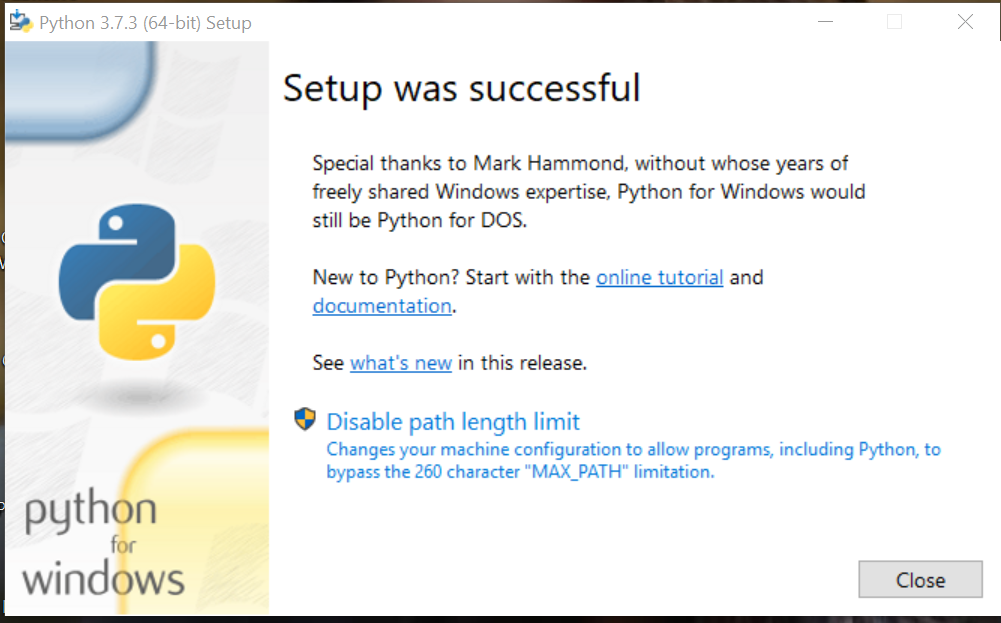
\includegraphics[scale=0.5]{figures/Capture3.PNG}
            \caption{Caption}
            \label{proses3}
        \end{figure}
    \end{itemize}
    
    \item Cara install pip 
    \begin{itemize}
        \item Download pip di instalasi dan klik kanan pada tulisan get.pp.py dan pilih save link as dan pilih tempat penyimpanan anda \ref{pip1}
        \begin{figure} [h]
            \centering
            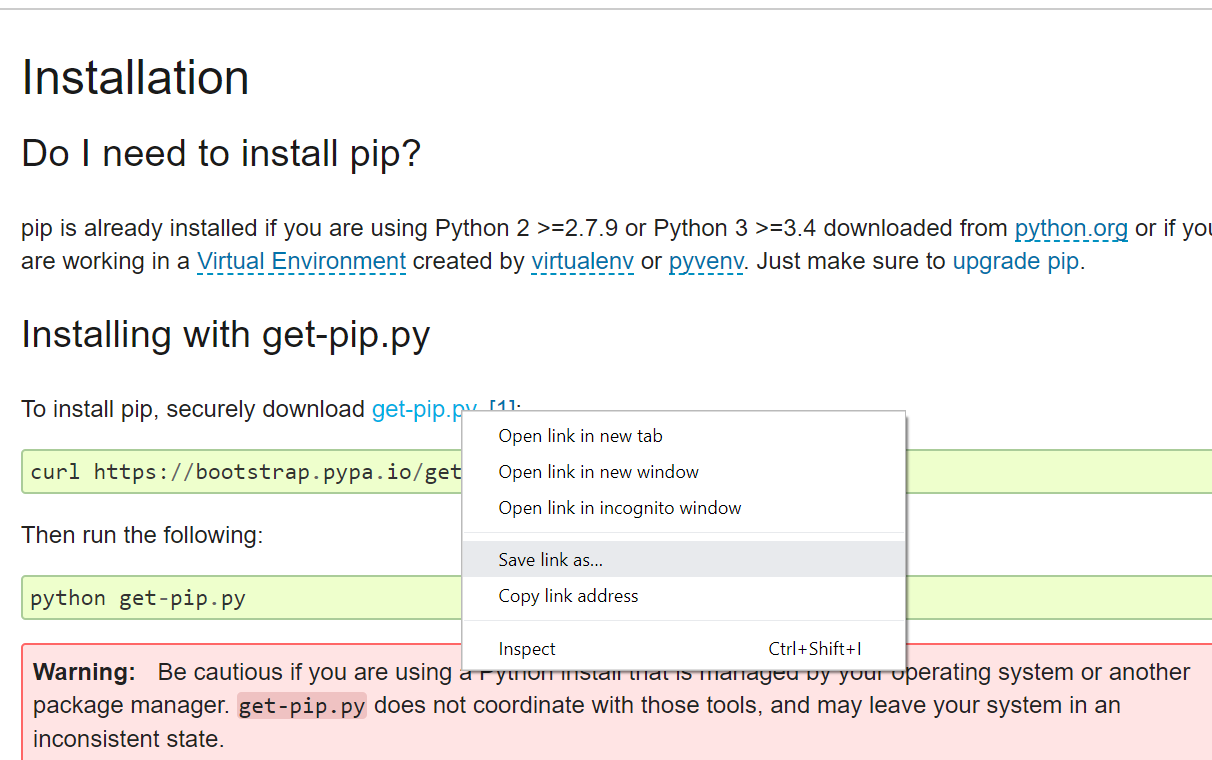
\includegraphics[scale=0.3]{figures/Screenshot (24).PNG}
            \caption{Caption}
            \label{pip1}
        \end{figure}
        
        \item Buka file yang tadi sudah di download lalu klik kanan open with pilih python \ref{pip2}
        \begin{figure} [h]
            \centering
            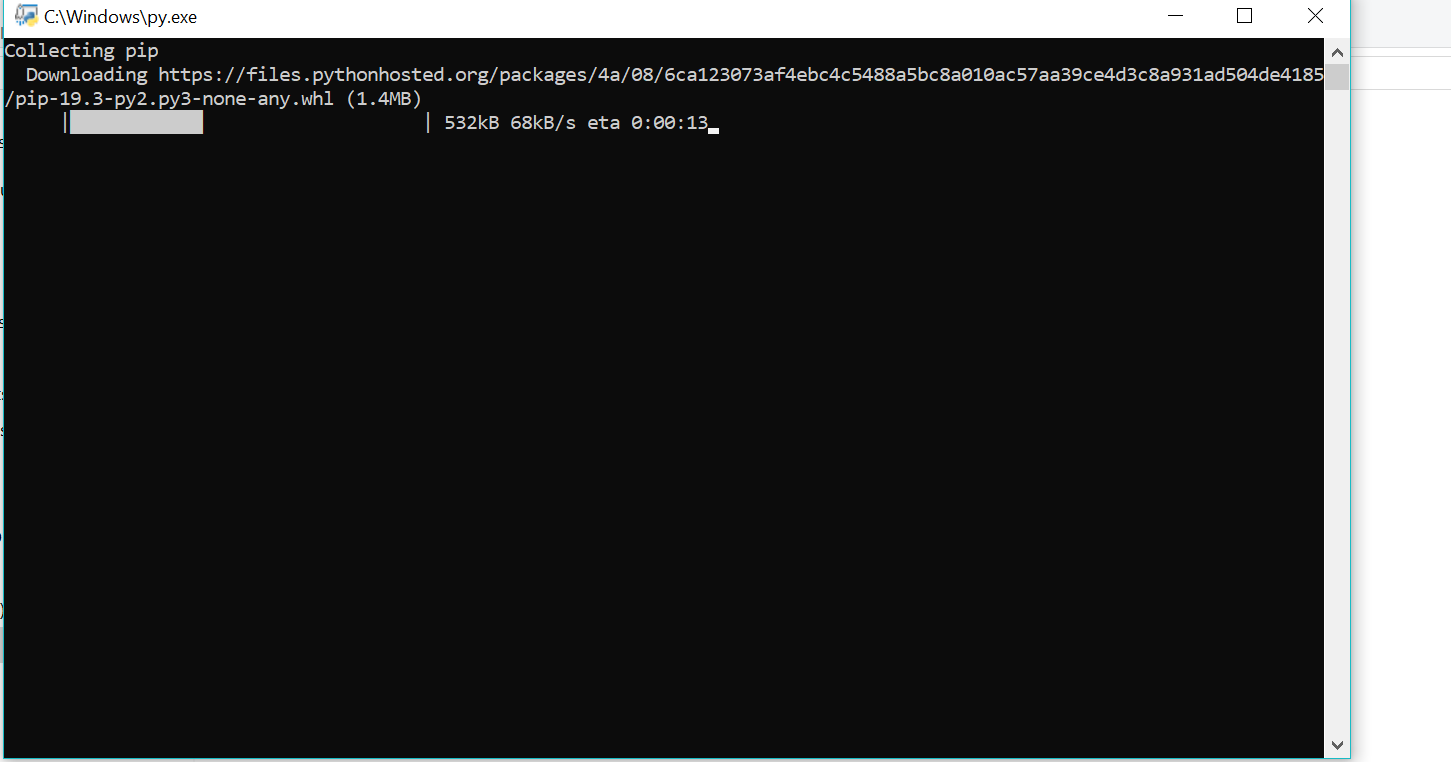
\includegraphics[scale=0.3]{figures/Screenshot (25).png}
            \caption{Caption}
            \label{pip2}
        \end{figure}
        
        \item Menunggu proses installasi sampai selesai \ref{pip3}
        \begin{figure} [h]
            \centering
            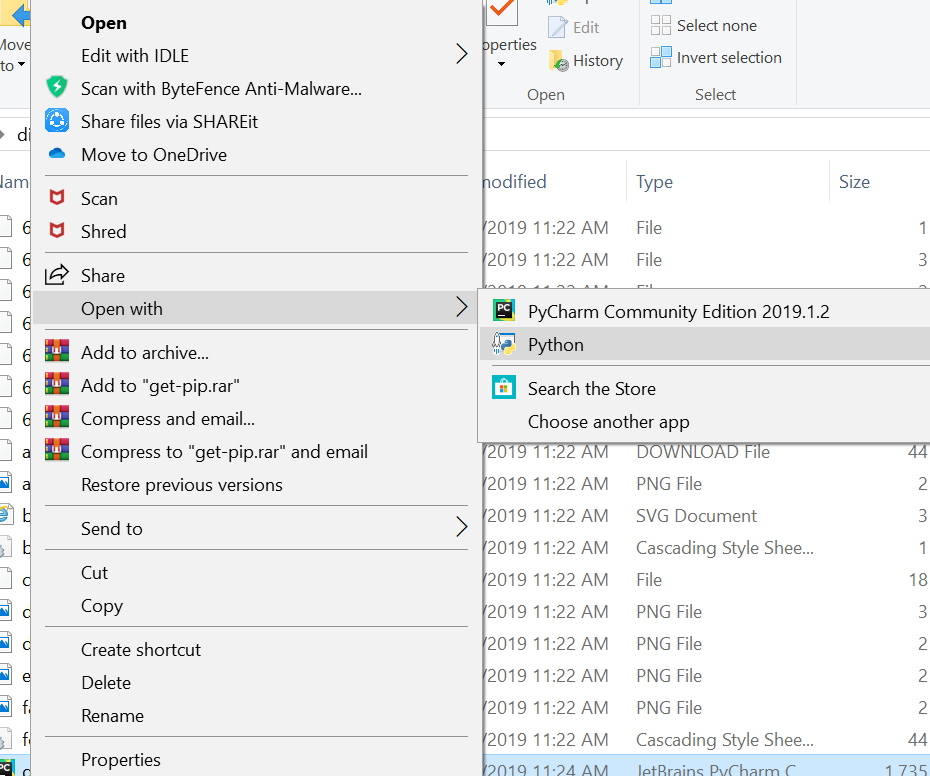
\includegraphics[scale=0.3]{figures/Screenshot (26).png}
            \caption{Caption}
            \label{pip3}
        \end{figure}
    \end{itemize}
    \item Cara setting environment
    \begin{itemize} 
        \item Buka control panel - system and security - system - Advance system setting\ref{capture5}
        \begin{figure} [h]
            \centering
            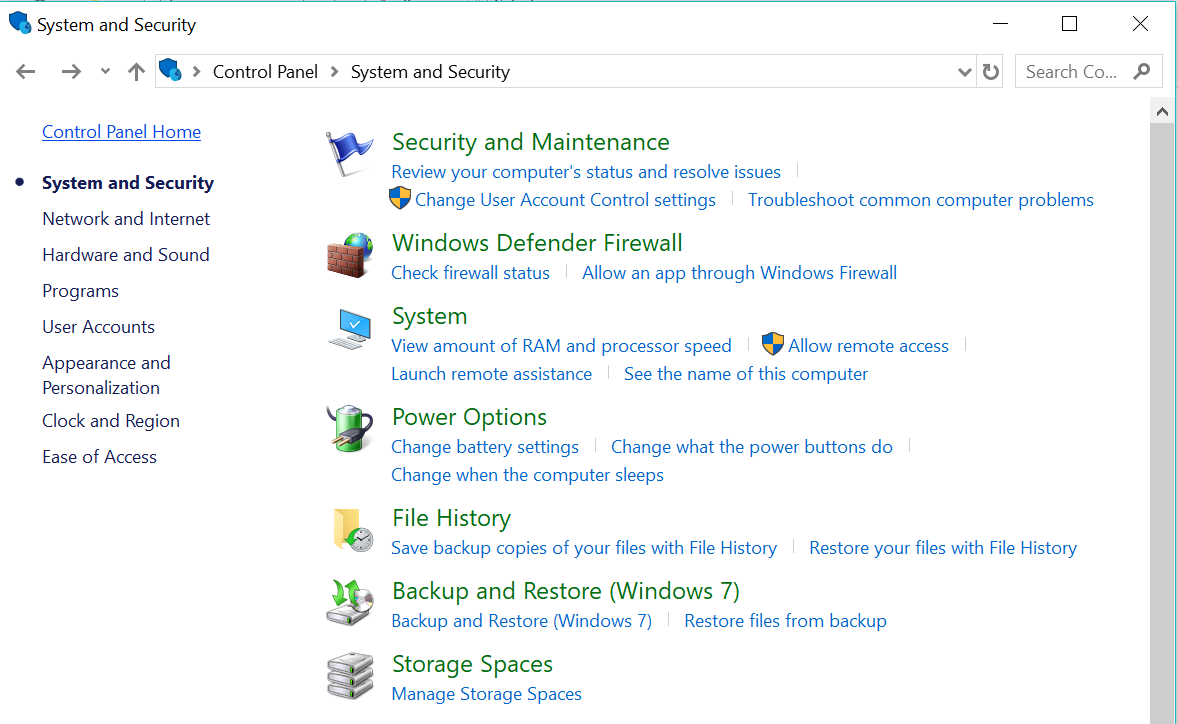
\includegraphics[scale=0.3]{figures/Capture5.PNG}
            \caption{Caption}
            \label{capture5}
        \end{figure}
        
        \item Klik Environment Variables \ref{capture6}
        \begin{figure} [h]
            \centering
            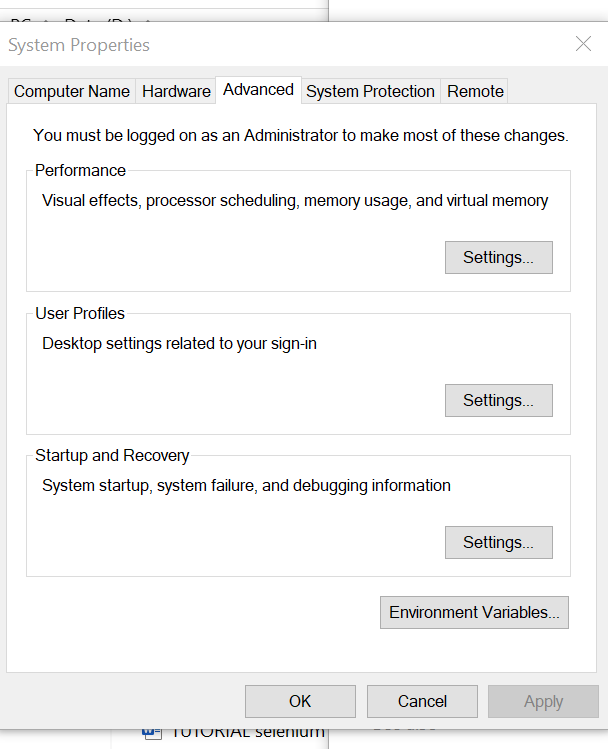
\includegraphics[scale=0.3]{figures/Capture6.PNG}
            \caption{Caption}
            \label{capture6}
        \end{figure}
        
        \item Pada bagian system variables scroll sampai ketemu path dan klik lalu akan ada system edit \ref{capture7}
         \begin{figure} [h]
            \centering
            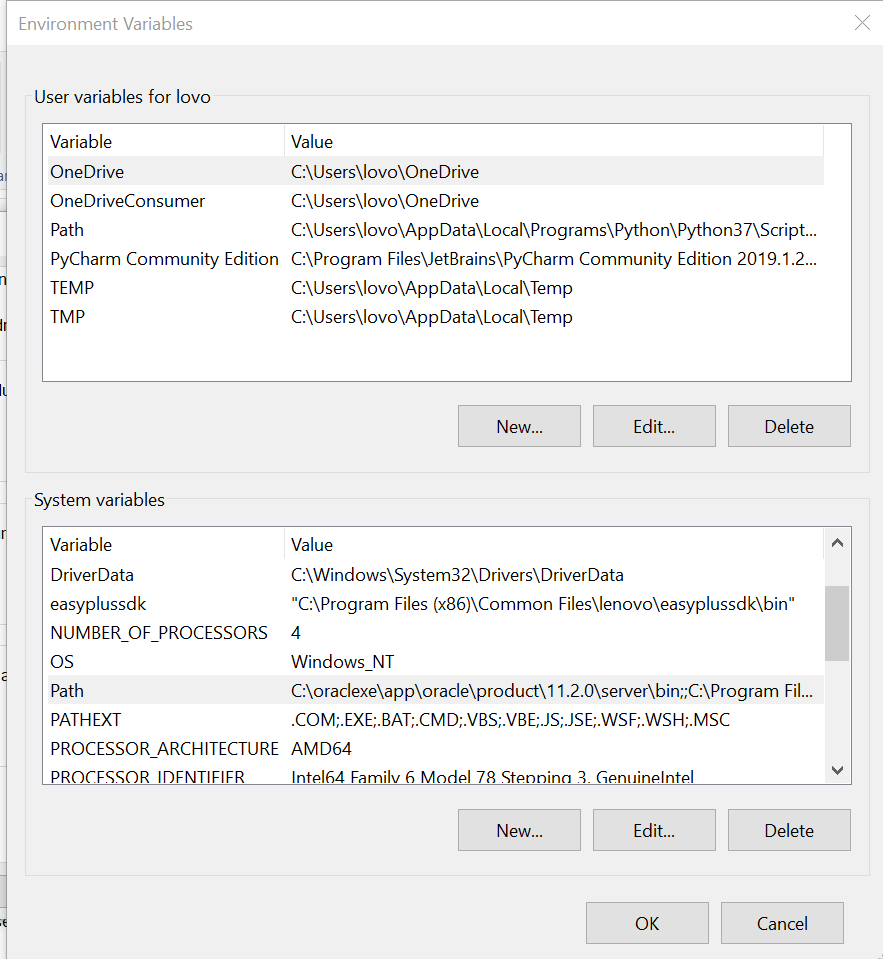
\includegraphics[scale=0.3]{figures/Capture7.PNG}
            \caption{Caption}
            \label{capture7}
        \end{figure}
        
        \item di belakang directory tambahkan ;C:\Python37\ tergantung versi python kalian dan klik ok semuanya \ref{capture8}
        \begin{figure} [h]
            \centering
            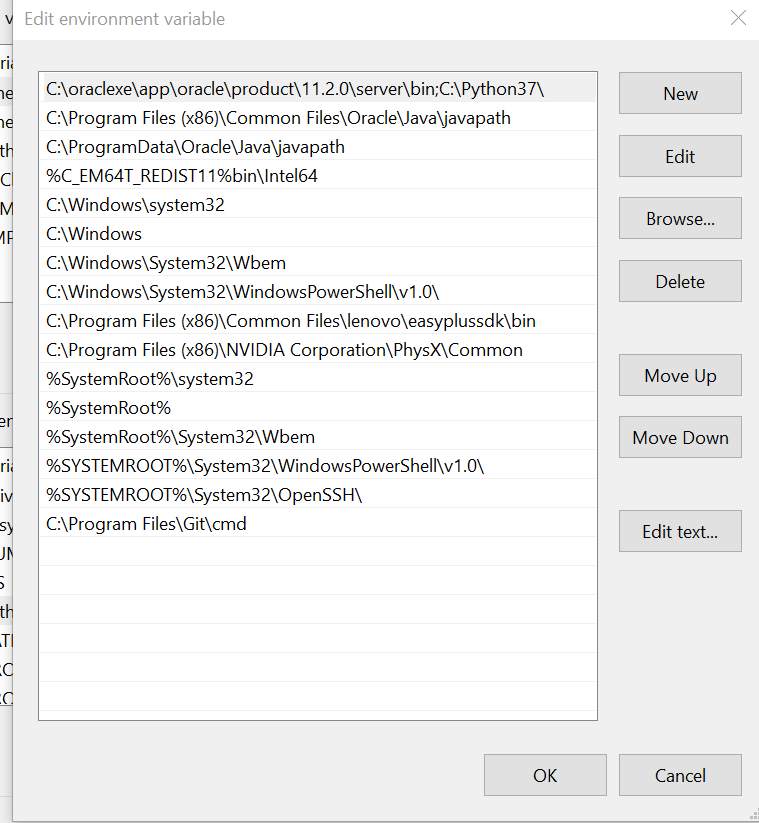
\includegraphics[scale=0.3]{figures/Capture8.PNG}
            \caption{Caption}
            \label{capture8}
        \end{figure}
        
        \item Buka cmd lalu ketikkan pip install request \ref{capture9}
        \begin{figure} [h]
            \centering
            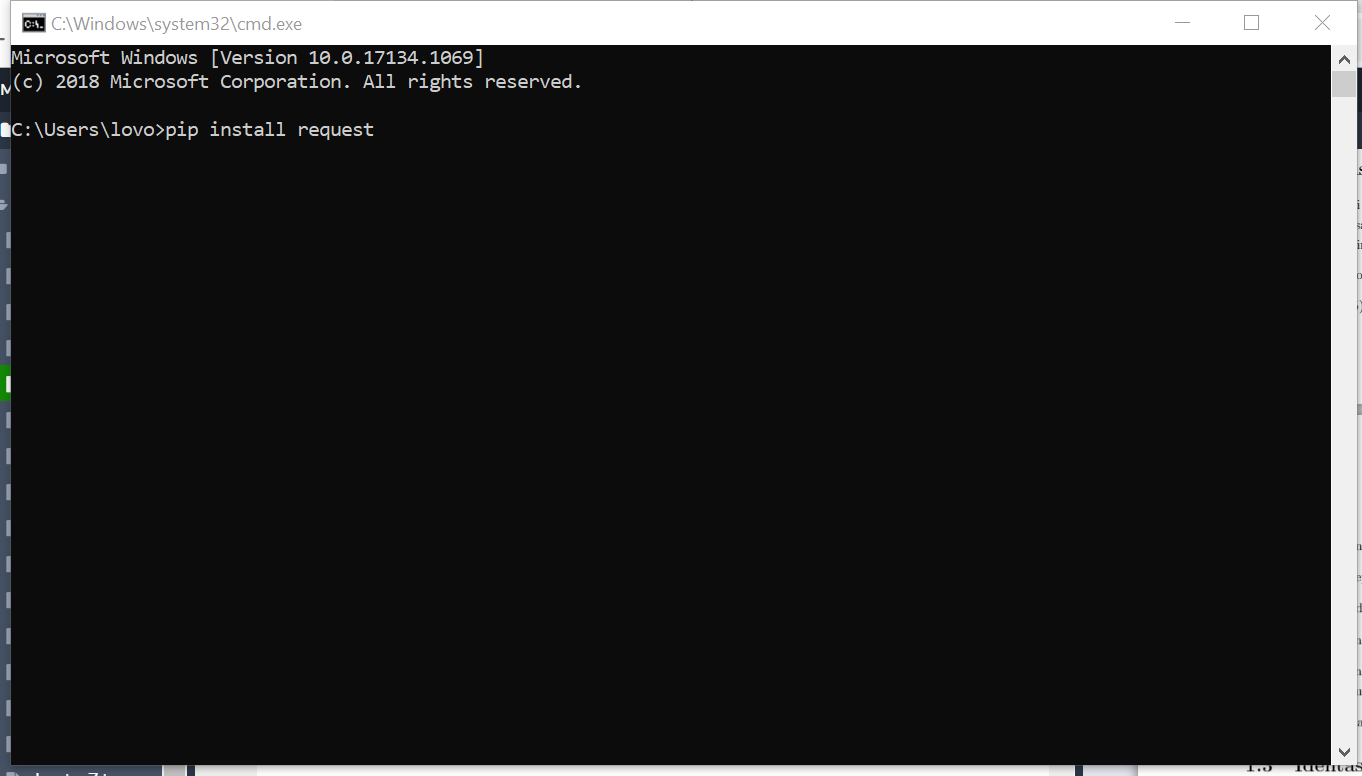
\includegraphics[scale=0.3]{figures/Capture9.PNG}
            \caption{Caption}
            \label{capture9}
        \end{figure}
        
        \item SELESAI \ref{capture10}
        \begin{figure} [h]
            \centering
            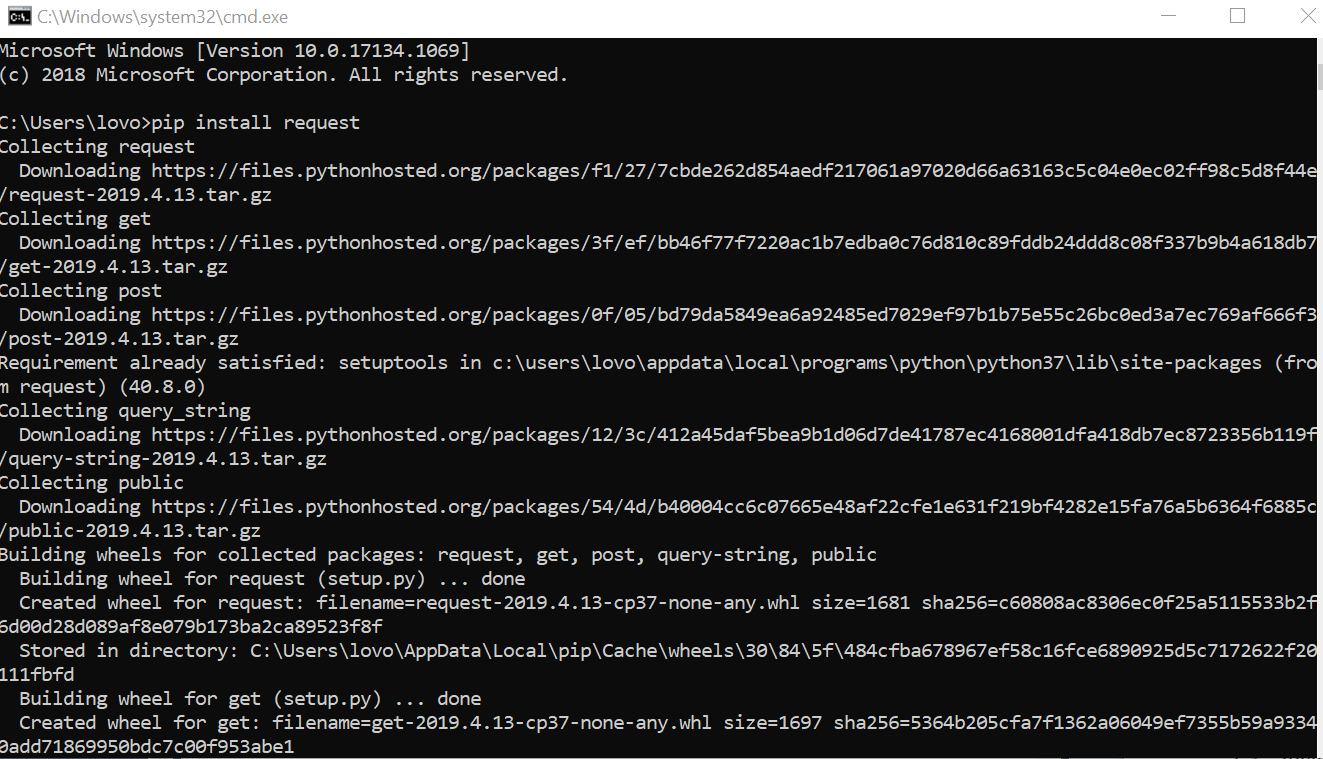
\includegraphics[scale=0.3]{figures/Capture10.PNG}
            \caption{Caption}
            \label{capture10}
        \end{figure}
    \end{itemize}
    
    \item mencoba entrepreter/cli melalui terminal atau cmd windows \ref{capture11}
    \begin{figure} [h]
            \centering
            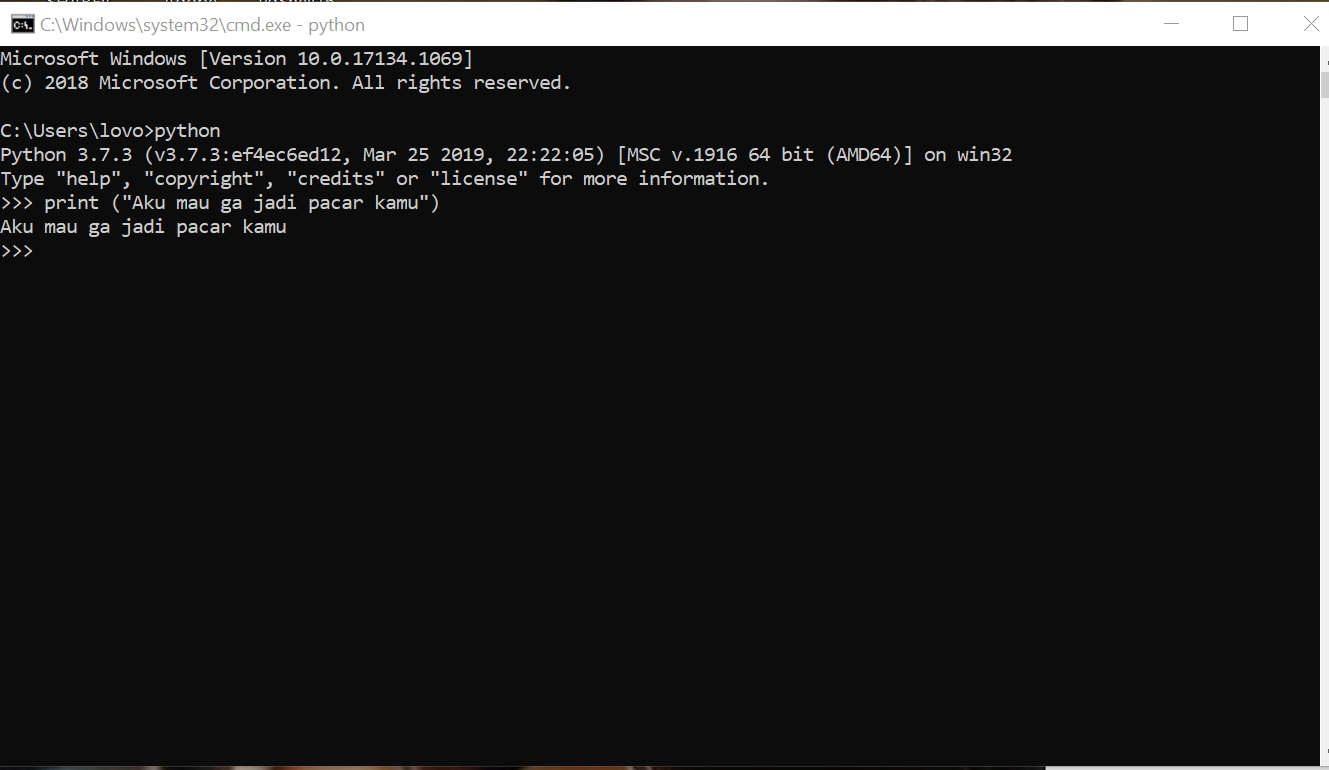
\includegraphics[scale=0.3]{figures/Capture11.PNG}
            \caption{Caption}
            \label{capture11}
        \end{figure}
        \item Menjalankan dan mengupdate anaconda dan spyder 
        \begin{itemize}
            \item Buka Anaconda Navigator yang telah di install lalu klik LAUNCH pada spyder \ref{capture12}
        \begin{figure} [h]
            \centering
            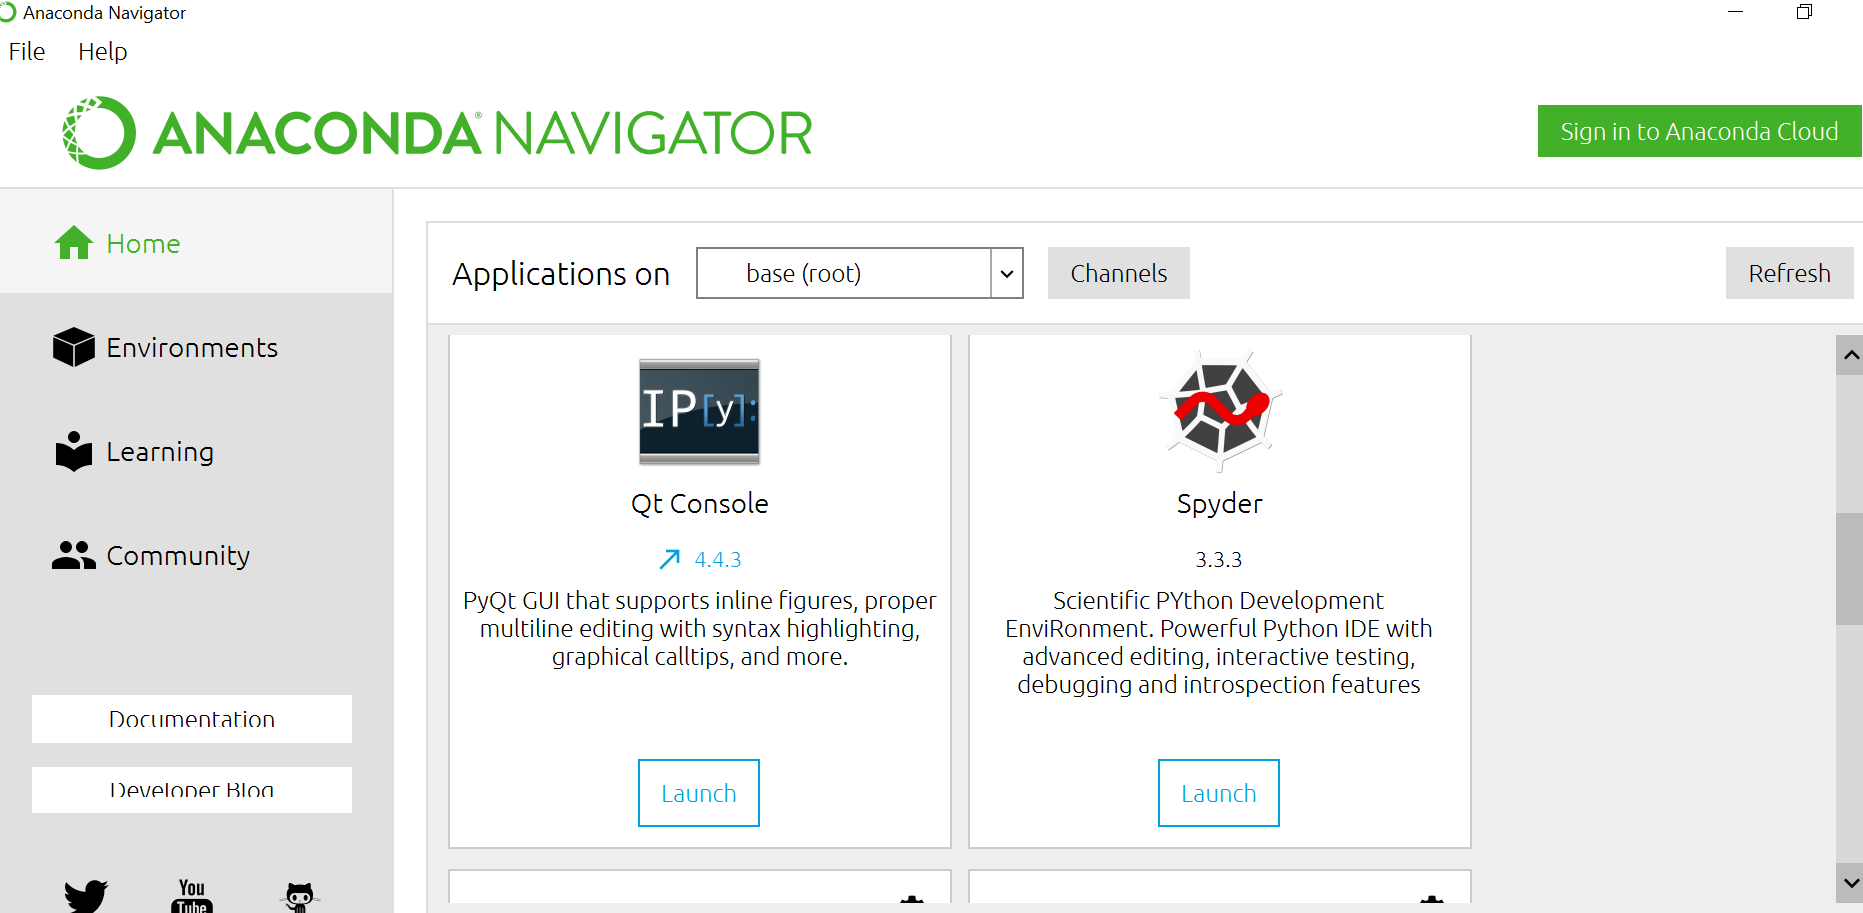
\includegraphics[scale=0.3]{figures/Capture12.PNG}
            \caption{Caption}
            \label{capture12}
        \end{figure}
        \end{itemize}
        
        \item  Cara menjalankan Script hello word di spyder 
        \begin{itemize}
            \item Buka spyder lalu masukkan script print('hello world'), kemudian run \ref{capture14}
             \begin{figure}
            \centering
            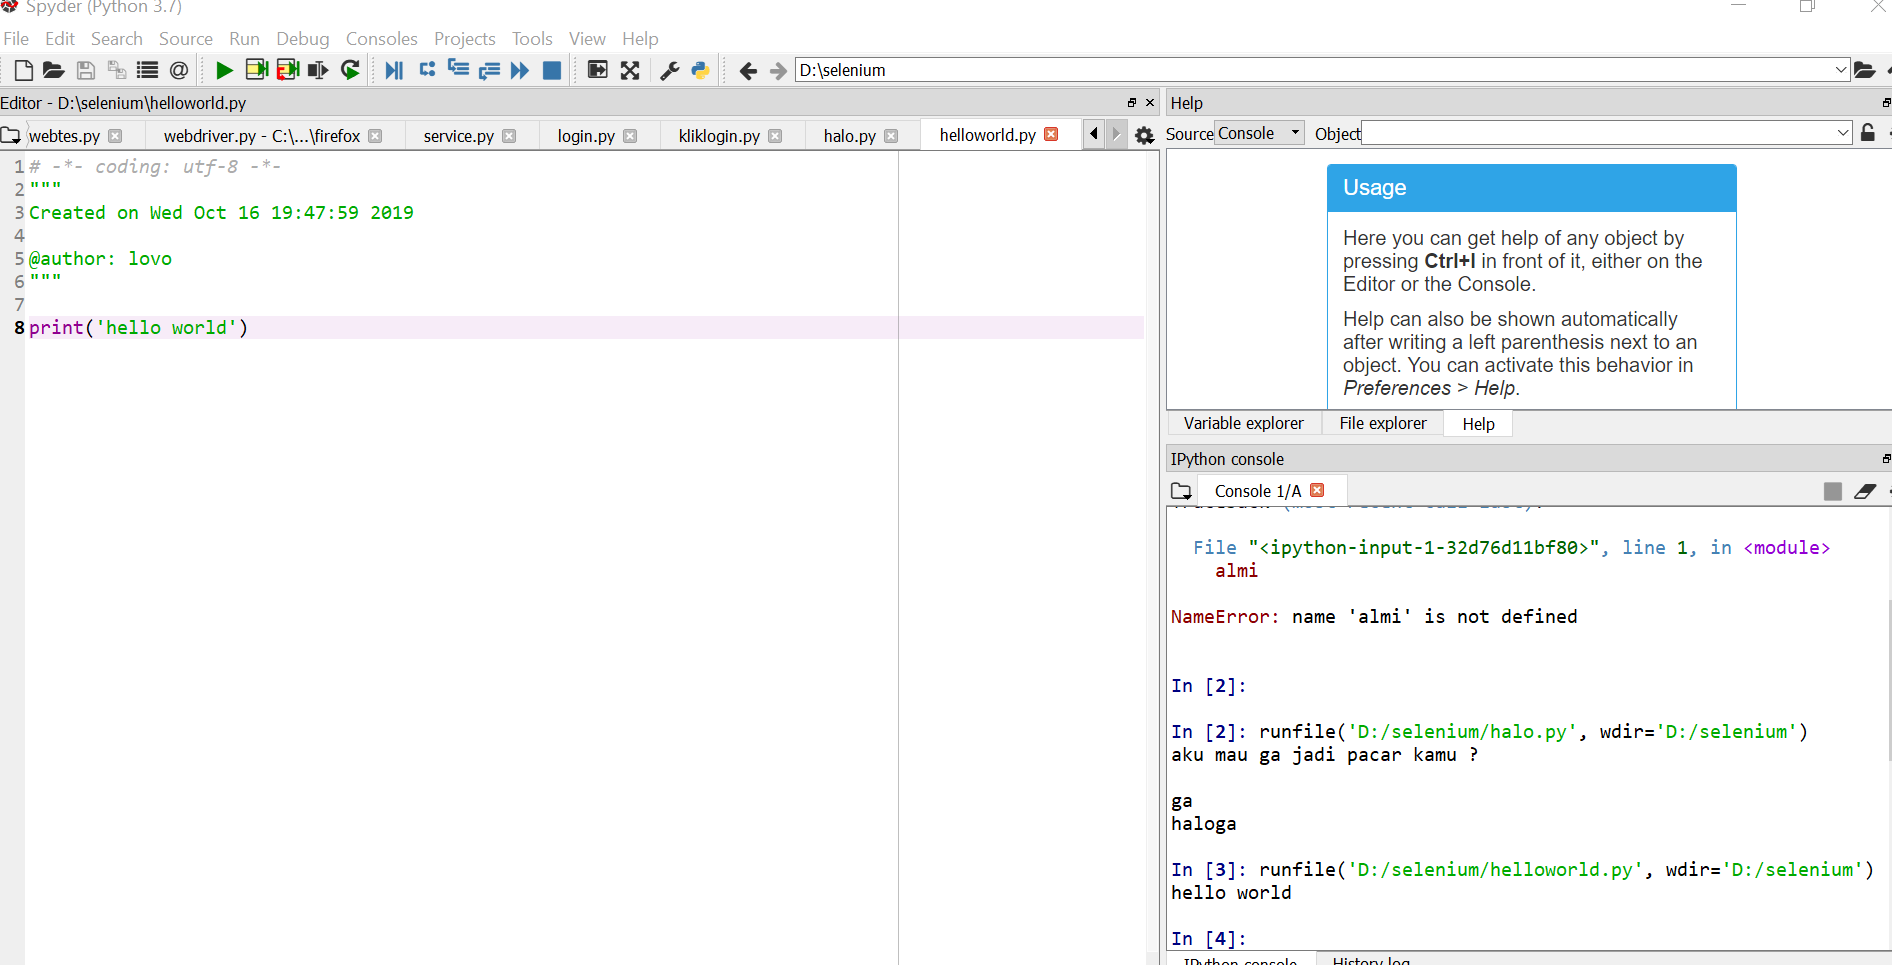
\includegraphics[scale=0.3]{figures/Capture14.PNG}
            \caption{Caption}
            \label{capture14}
        \end{figure}
        \end{itemize}
        
        \item Cara menjalankan Script otomatis login aplikasi akademik dengan library selenium dan inputan user
        \begin{itemize}
            \item Masuk spyder lalu masukkan scriptnya lalu klik run \ref{capture16}
            \begin{figure} [h]
                \centering
                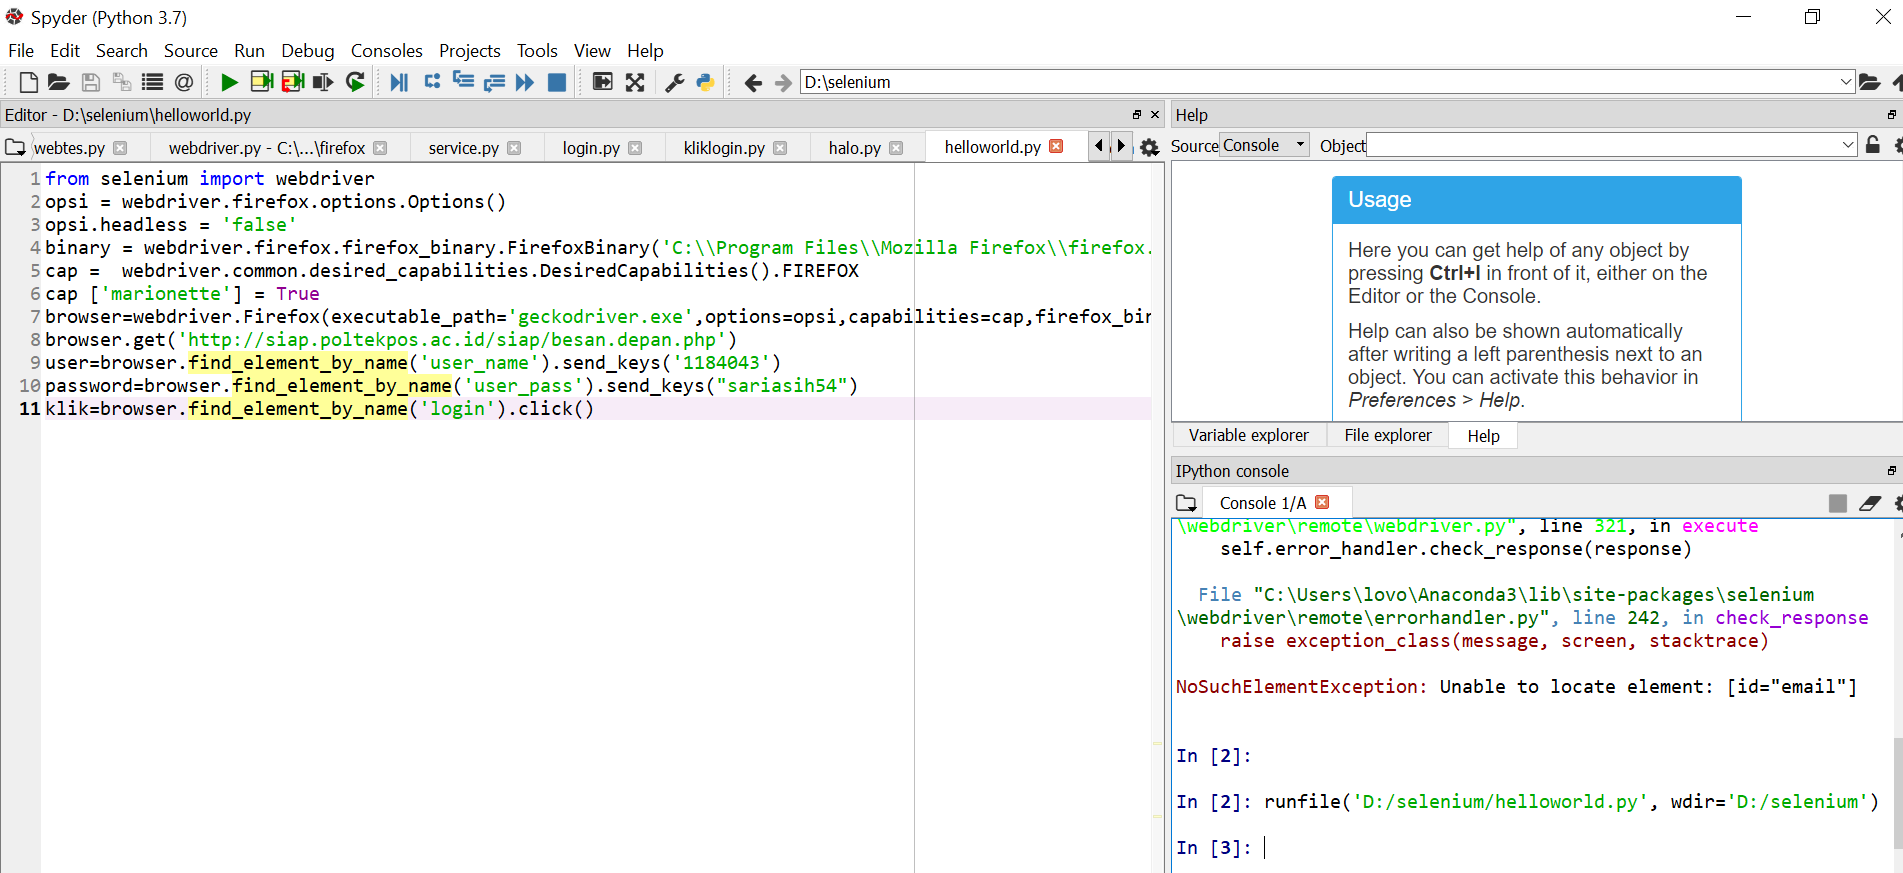
\includegraphics[scale=0.3]{figures/Capture16.PNG}
                \caption{Caption}
                \label{capture16}
            \end{figure}
            
            \item Secara otomatis masuk ke halaman aplikasi akademik \ref{capture17}
            \begin{figure} [h]
                \centering
                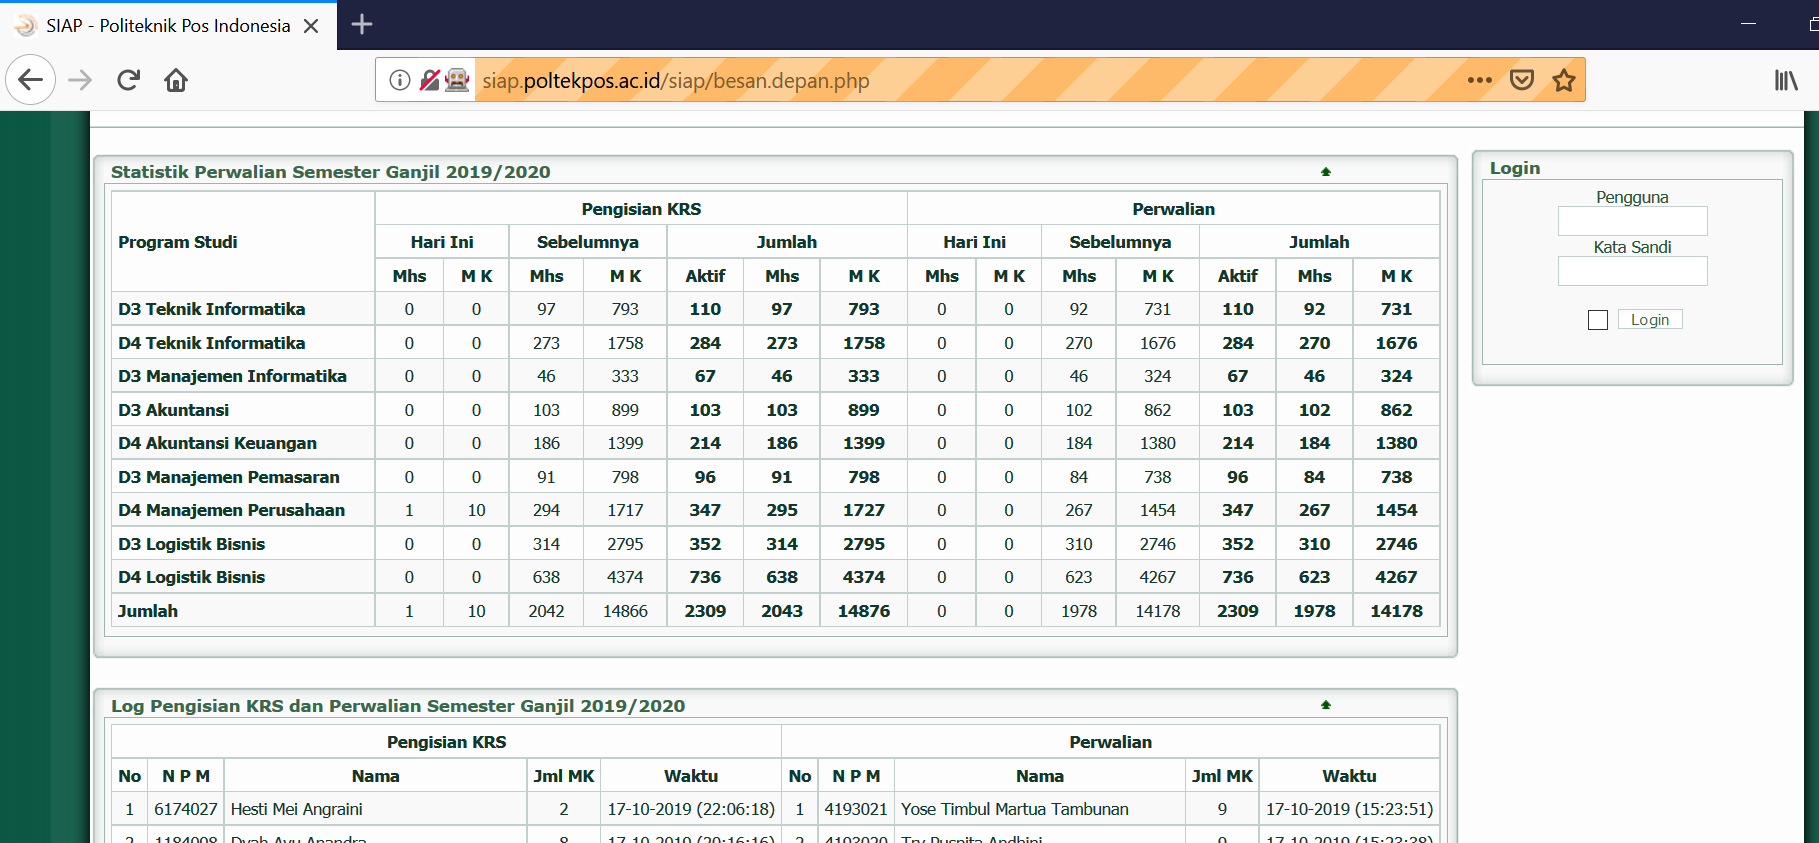
\includegraphics[scale=0.3]{figures/Capture17.PNG}
                \caption{Caption}
                \label{capture17}
            \end{figure}
            
            \item Secara otomatis juga login ke aplikasi akademik \ref{capture18}
             \begin{figure} [h]
                \centering
                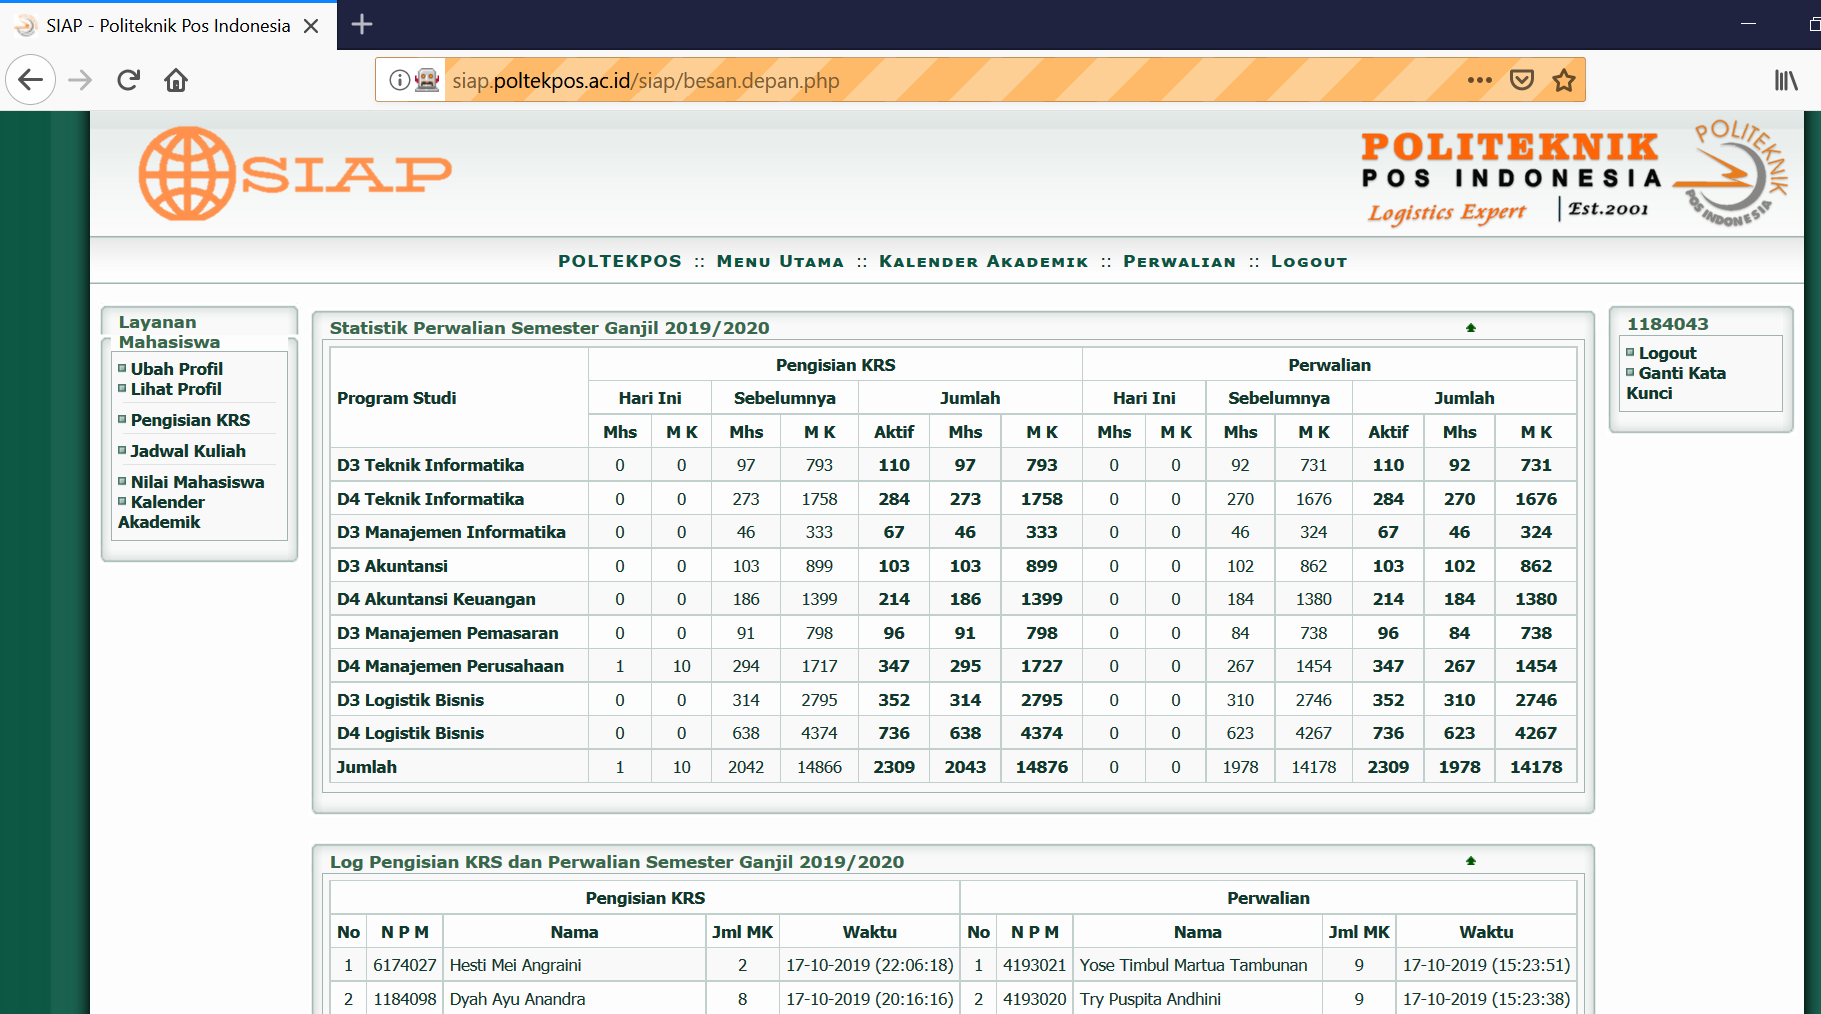
\includegraphics[scale=0.3]{figures/Capture18.PNG}
                \caption{Caption}
                \label{capture18}
            \end{figure}
        \end{itemize}
        \item Cara pemakaian variable explorer di spyder \ref{capture15}
         \begin{figure} [h]
            \centering
            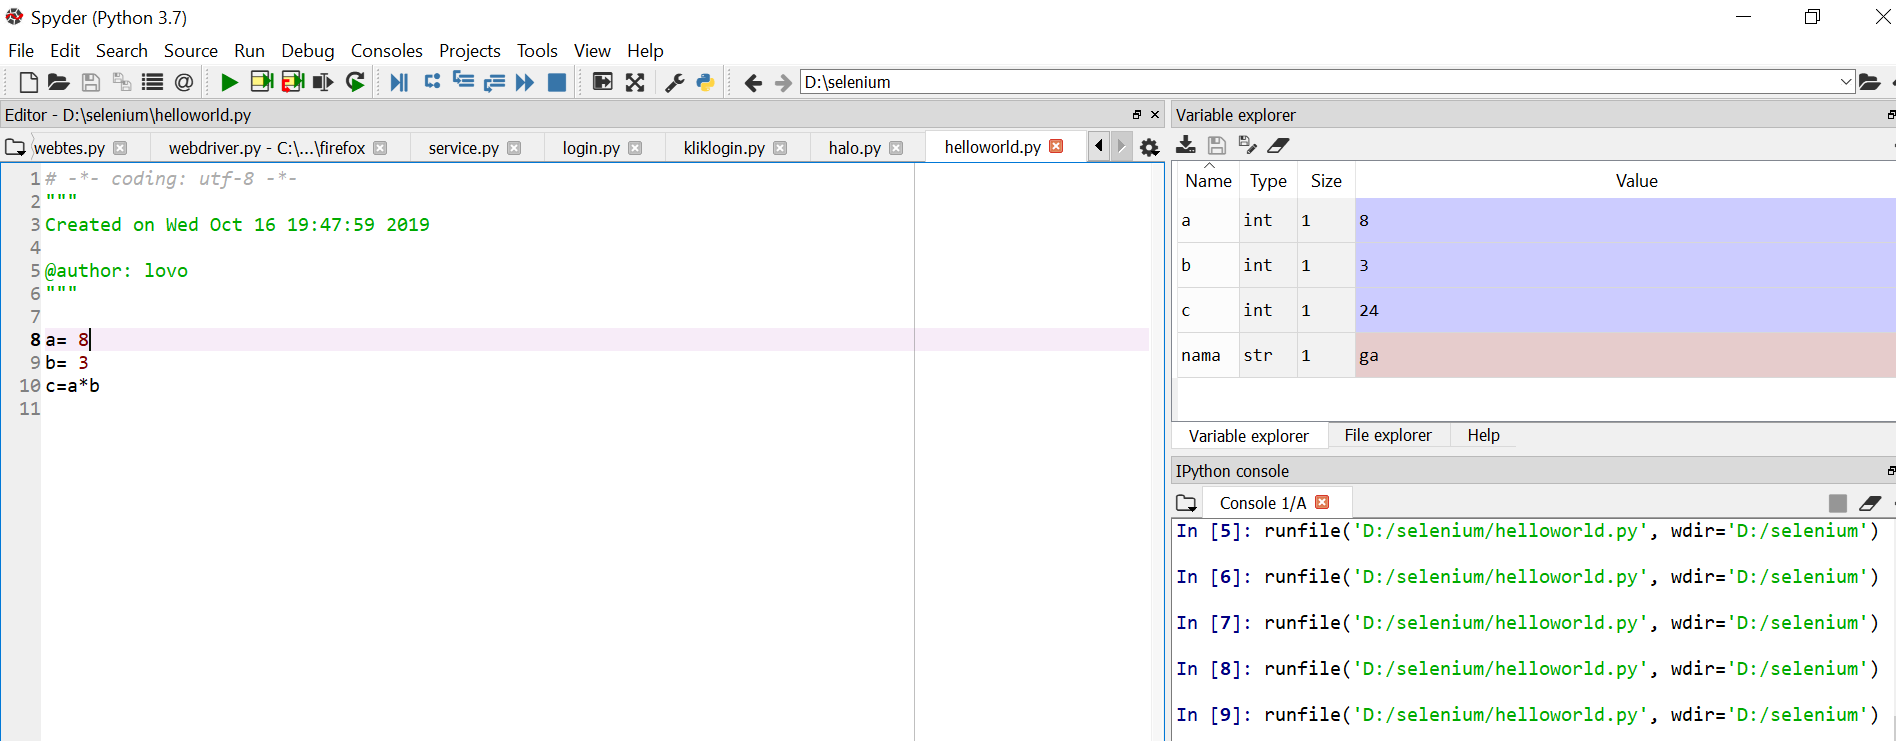
\includegraphics[scale=0.3]{figures/Capture15.PNG}
            \caption{Caption}
            \label{capture15}
        \end{figure}
        
    \textbf{Identasi}
        \begin{enumerate}
        
        \item  Penjelasan Identasi 
         Identasi ( tulisan yang menjorok kedalam) adalah suatu blok kode di python untuk menandai blok/grup kode.  Jumlah spasi untuk setiap baris yang ada dalam satu blok kode harus sama. 
        
       \end{enumerate}
        
\end{enumerate}
        